\begin{frame}
\frametitle{Uniform Buffer: Demo}
\begin{figure}[ht]
    \centering
    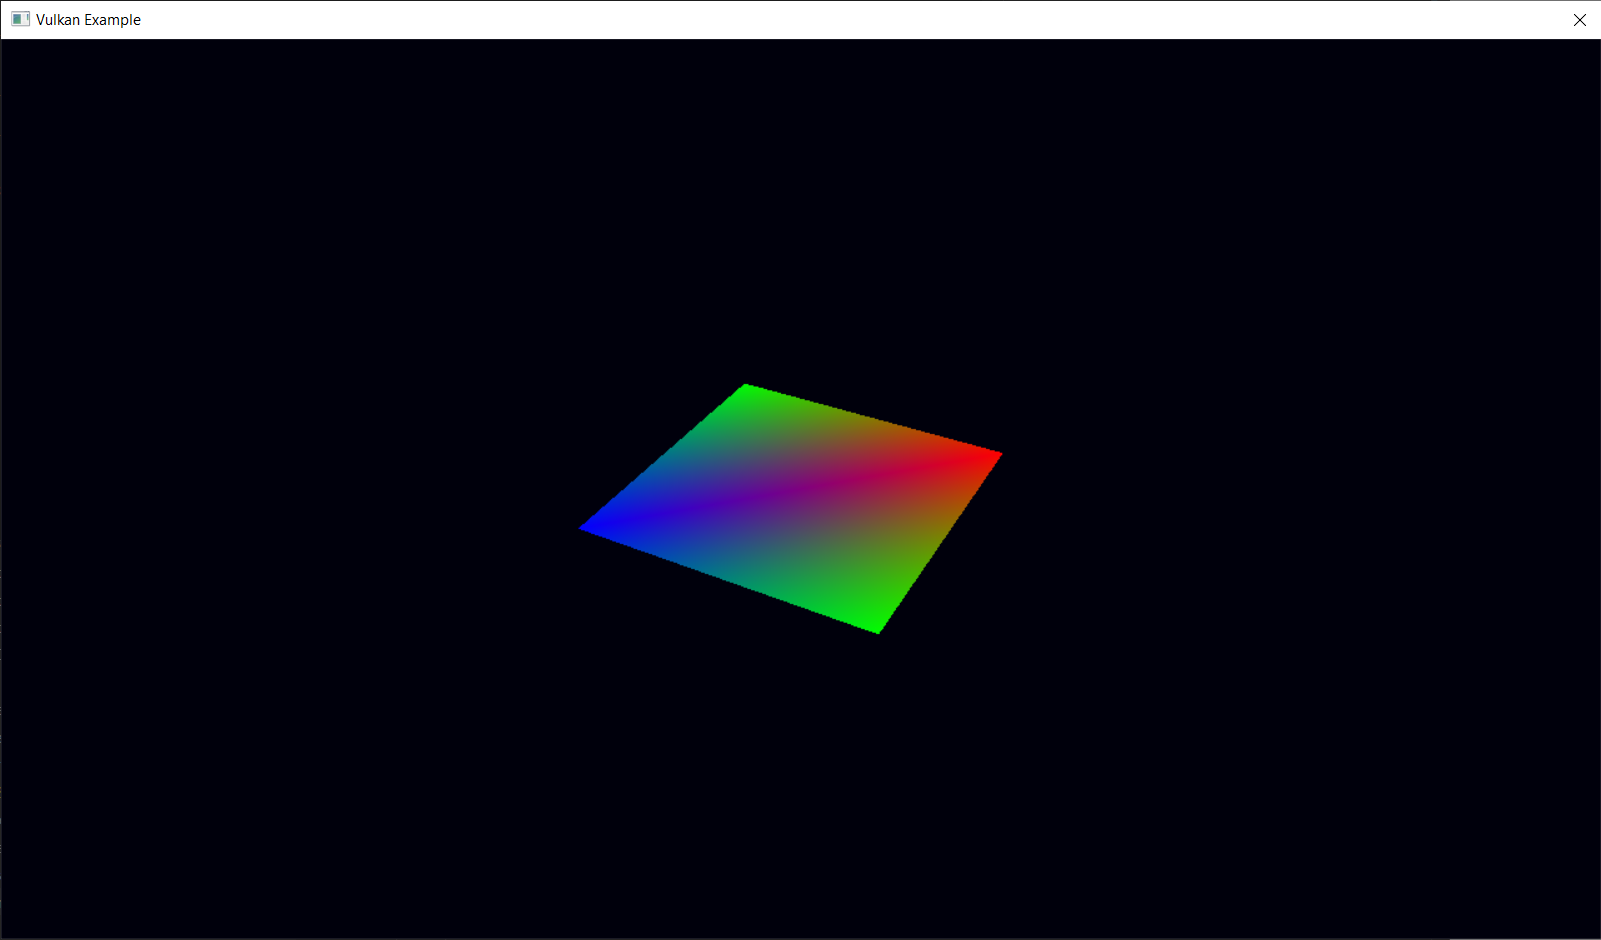
\includegraphics[scale=0.25]{images/SlidesUniforms/RenderQuad.png}
\end{figure}
\end{frame}

\begin{frame}
\frametitle{Uniform Buffer}
\begin{itemize}
\item Una variabile globale di uno shader è detta uniform
\item Passiamo le variabili globali agli shader usando uno uniform buffer
\item Siccome tali variabili cambiano frequentemente, allochiamo uno uniform buffer su memoria della GPU host visible
\item Creiamo un pipeline layout object
\item Un pipeline layout object descrive quali descriptor sono accessibili in quali shader
\item Creiamo un descriptor set layout
\item Un descriptor set layout descrive il contenuto di un descriptor set
\item Creiamo un descriptor set basandoci sul descriptor set layout
\end{itemize}
\end{frame}
